 \chapter{Introduction}
\label{cp.intro}

From ancient times to the modern day, astronomy has played an essential role in all cultures and eras.
Questions about the infinite cosmos and our place in it have intrigued great minds for millennia.
To answer these questions, astronomers construct instruments to tap into the cosmos' ocean of data and devise statistical methods to make inferences.
Each drop of cosmic data improves inference and takes us to the answers we seek.
However, until quite recently, astronomy has existed in a relatively data-poor environment. 
Now, with the assistance of computers and sophisticated instruments, astronomers have access to massive datasets not easily described by traditional methods.
In response, some astronomers are turning to data-driven approaches to make inferences with the vast quantities of newly acquired data .
This section takes a look back at areas of astronomy that have recently seen significant data improvements and have provided new insights into the nature of stars, planets, and even black holes.
These conversations will spark ideas and provide impetus for the rest of the thesis.


\section{Observational HR-Diagrams through the ages}

In 1872, astronomers began recording spectroscopic data for thousands of stars in the Henry Draper Catalogue~\citeme.
Antonia Maury, a female astronomer, working in the Harvard observatory, noticed that some stars in the catalog were much brighter than other stars of the same color and sorted those brighter stars into a different category from their less-luminous brethren. 
Several years later, Einjar Hertzpsrung, working on his star classification project in 1905, noticed the same thing as Maury: some stars had very similar colors but very different brightness~\citeme.
With more data available in 1913, Henry Norris Russell demonstrated the effect far more strikingly. 
Russel plotted the absolute magnitude against spectral type for Maury's stars, nearby stars with parallaxes measured at the time, stars from the open cluster Hyades, and several moving groups ($\sim200$ stars in total). 
This plot, an observational Hertzpsrung-Russel (HR) diagram, has been recreated with modern stellar data in Figure~\ref{fig:HR-diagrams}a.

\begin{figure}
\begin{center}
  \centerline{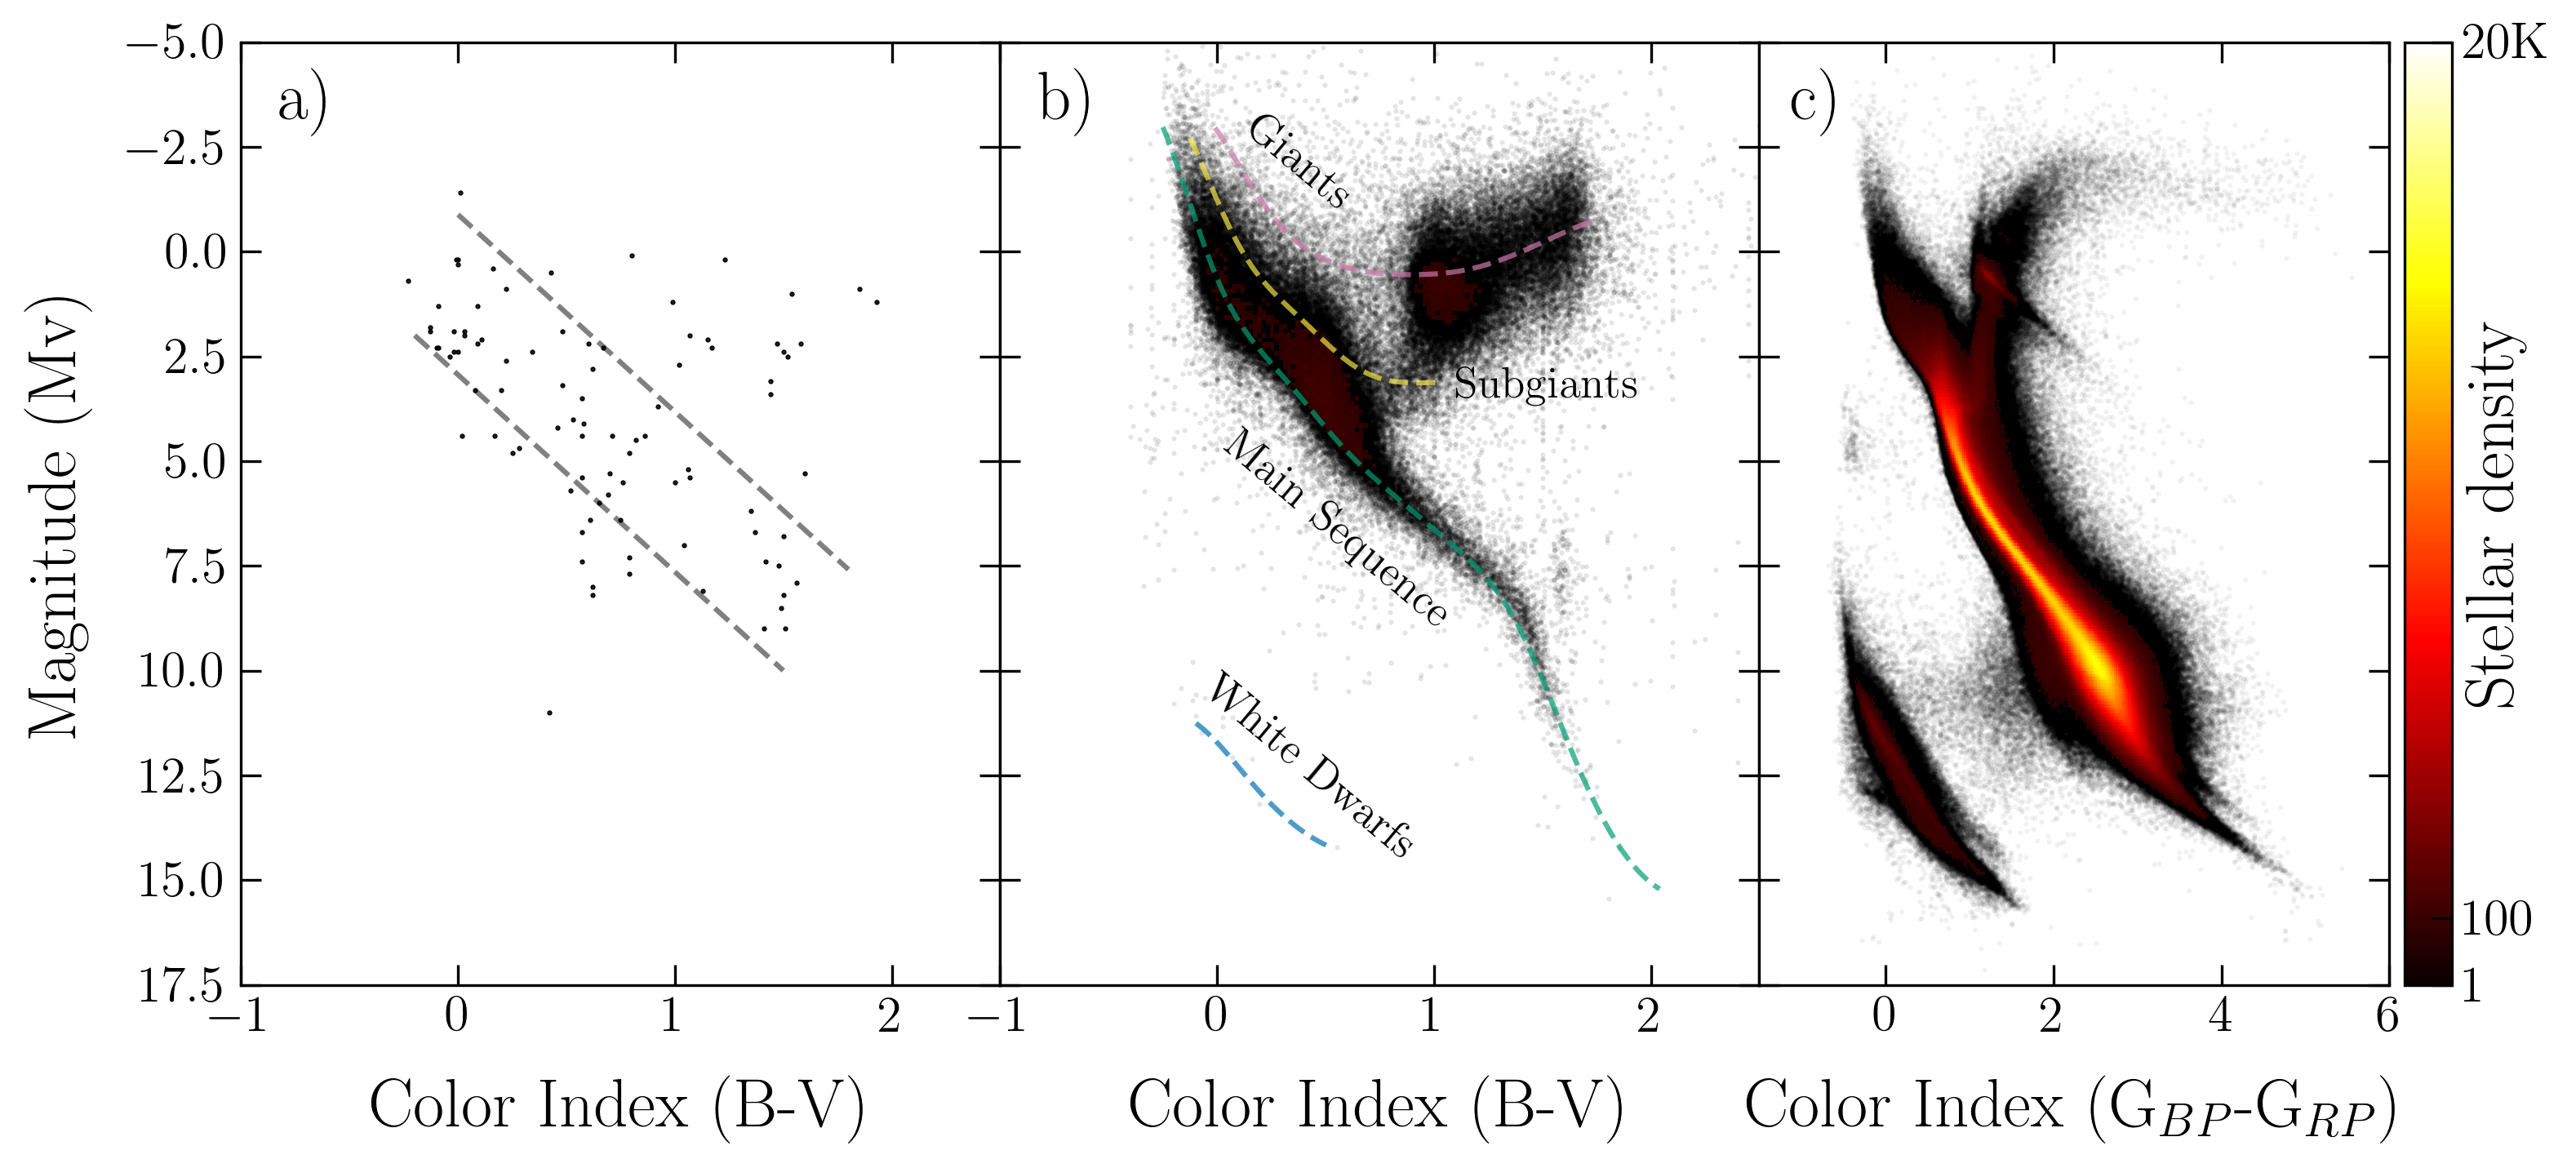
\includegraphics[width=1.2\linewidth]{figures/hr_diagram.png}}
  \caption{\textbf{Observational HR-Diagrams through the ages: Catalog stars' color index plotted on the horizontal axis and absolute magnitude on the vertical axis. Different regions of the diagram depend on the stars' masses, chemical composition, ages, and stages in the stellar life cycle. The color scale represents the number of stars in each portion of the diagram (black represents lower numbers of stars, and brighter colors correspond to increasingly higher numbers of stars). Panel (a) uses stars cataloged in 1914, panel (b) uses 1993 Hipparcos stars, and panel (c) uses 2022 Gaia stars. 
}  \github{https://github.com/avivajpeyi/hr_diagram_past_to_present}}
  \label{fig:HR-diagrams}
\end{center}
\end{figure}

The plot's data points helped Russell demonstrate that the temperature and luminosity of stars are related.
Brighter stars are displayed in the top part of the diagram, while dimmer stars are in the bottom. 
Bluer (hotter-surface) stars are on the left, and redder (cooler-surface) stars are on the right. 
Russell noted that most of the plotted stars fell in a band from the upper left to the lower right.
He indicated this region with lines (the gray dashed lines reconstructed Figure~\ref{fig:HR-diagrams}a).
Russell and Hertzsprung also noticed a separate category of bright but cool red stars in the upper right corner. 
They realized that these bright-cool red stars have a large surface area to produce high luminosity at low temperatures. 
Hertzsprung hence dubbed these as the ``giant" stars.  
Consequently, he named the less-luminous low-temperature red stars "dwarf" stars. 
Russell recognized that the red dwarfs were just the bottom end of the band of stars within the gray lines in Figure~\ref{fig:HR-diagrams}a. 
Hence, Russell extended the grouping of ``dwarf" stars to the entire sequence, the sequence now known as the ``main sequence."
Even though the plot only contained a few stars, it provided Russell with a convenient way to illustrate his ideas about stellar evolution:
\myblockquote{The giant stars then represent successive stages in the heating up of a body and must be
more primitive the redder they are; the dwarf stars represent consecutive stages in later
cooling, and the reddest of these are the farthest advanced.}{Henry Russell, 1914}

  % https://arxiv.org/pdf/1302.0862.pdf
Other astronomers like Eddington also used similar data and the HR diagram to drive some of their theories. 
For example, a decade later, Eddington's mass-luminosity relation would add evidence for stellar evolution down the main sequence.
Soon, the HR diagram became a cornerstone diagram for modern astrophysics, and the concepts of stellar categories led to various advancements in our understanding of stellar physics~\citeme. 
Fortunately, since 1914, technological advances have created much larger samples of stars with well-measured properties, further improving our understanding of stellar physics.


The European Space Agency launched Hipparcos Satellite in 1989\footnote{Hipparcos, an acronym for HIgh Precision PARallax COllecting Satellite, is also reference to Hipparchus, the ancient Greek astronomer who drew up the first accurate star map.}. 
One of the Hipparcos mission's primary goals was to provide a higher resolution observational HR diagram to obtain a detailed structure of stars with $M_v>0$ magnitude. 
In its four years of operation, this satellite cataloged nearly 120,000 stars. 
The Hipparcos catalog stars with low parallax errors, plotted in Figure~\ref{fig:HR-diagrams}b,  show many more details than those in the 1914 HR diagram. 
Firstly, the vertical arm leading off the main sequence and turning to the right is much better defined -- this is the red giant branch indicating that as massive stars get older, they swell and become brighter and redder.
Similarly, the lower left of the diagram shows the white dwarf branch. 
The white dwarf region displays where the less massive stars (like our sun) that cannot undergo a supernova as they get older end up. 
Additionally, if we plotted stars with higher parallax errors, various other categories, such as the bright and super giants, are also visible.

A few years later, Hipparcos's successor Gaia made a considerable leap by cataloging 1.8 billion stars at an accuracy 200 times better than that of Hipparcos. 
Figure~\ref{fig:HR-diagrams}c displays the Gaia stars with low parallax errors obtained in Gaia's third data release. 
This new HR diagram contains over 100 times more stars than Hippacros and allows astronomers to identify more refined details. 
For example, compare the hand full of white dwarfs in the Hipparcos diagram versus the thousands in the Gaia HR diagram.
This increase in white dwarf data has allowed astronomers to study the differences between white dwarfs made with helium cores and hydrogen cores ~\citeme. 
Another exciting detail displayed in the Gaia HR diagram is the imprint of stellar binaries.
These binaries are present both in the main sequence and the white dwarf regions of the diagram (see the second tails at slightly higher magnitudes in both the main sequence and white dwarf regions of the plot).
The Gaia HR diagram appears to have a smaller red giant branch compared to Hipparcos's HR diagram. However, the Gaia HR diagram has many more resolved features, such as the primary and secondary red clumps and the asymptotic giant branch bump. 
The sheer volume of the data made such discoveries possible! 

In addition to data on stellar temperatures and brightness, our catalogs now also contain stellar spectra and time-series data on stellar positions and proper motions.
This data has enabled astronomers to drive theoretical work and make inferences about the nature of stars.
In the following two sections of this chapter, we discuss two more fields where astronomical data has unveiled profound discoveries. 



\section{The era of Gravitational wave astronomy}

%% What is a GW 
When some stars reach the end of their lives, they can turn into compact objects such as neutron stars and black holes. 
Some compact objects give away their positions via electromagnetic (EM) radiation due to accretion. 
Others reveal themselves via gravitational wave (GW) radiation emitted due to an oscillating mass quadrupole moment.
Any system with a gravitational quadrupole changing with time produces changes in its gravitational field, resulting in the emission of energy as gravitational waves.
Gravitational-wave astronomy gives us a new tool to examine the cosmos that complements classic electromagnetic astronomy.
Using gravitational waves, astronomers can research binary black holes and neutron stars that would otherwise be inaccessible.
However, it was only recently that astronomers were able to detect GWs. 

%% History of GW
In 1974, Russell Hulse and Joseph Taylor discovered a pulsar signal using the Arecibo radio telescope.
Measurements revealed that the pulsars' orbital period fluctuates repeatedly every few hours, indicating it is in orbit with a hidden companion.
Hulse and Taylor noted that the orbital period was decaying -- the pulsar and its companion were inspiralling.
After observing the system for another 30 years, they determined that the decrease of the orbital period was the result of the binary releasing gravitational waves, the first observation of gravitational waves.

This indirect detection of gravitational waves paved the groundwork for the Laser Interferometer Gravitational-Wave Observatory, LIGO. 
LIGO was constructed in 1999, but it was not until 2014 that the first gravitational wave from the merging of a binary black hole system was identified.
Since then, the LIGO-VIRGO-KAGRA (LVK) collaboration has recorded several petabytes of data and astronomers have discovered more than ninety gravitational wave (GW) signals from compact binary mergers.
Individually, these events have provided astronomers with interesting information about various astrophysical objects. 
Taken together, the events form a population that can be studied as a whole. 

\begin{figure}
\begin{center}
  \centerline{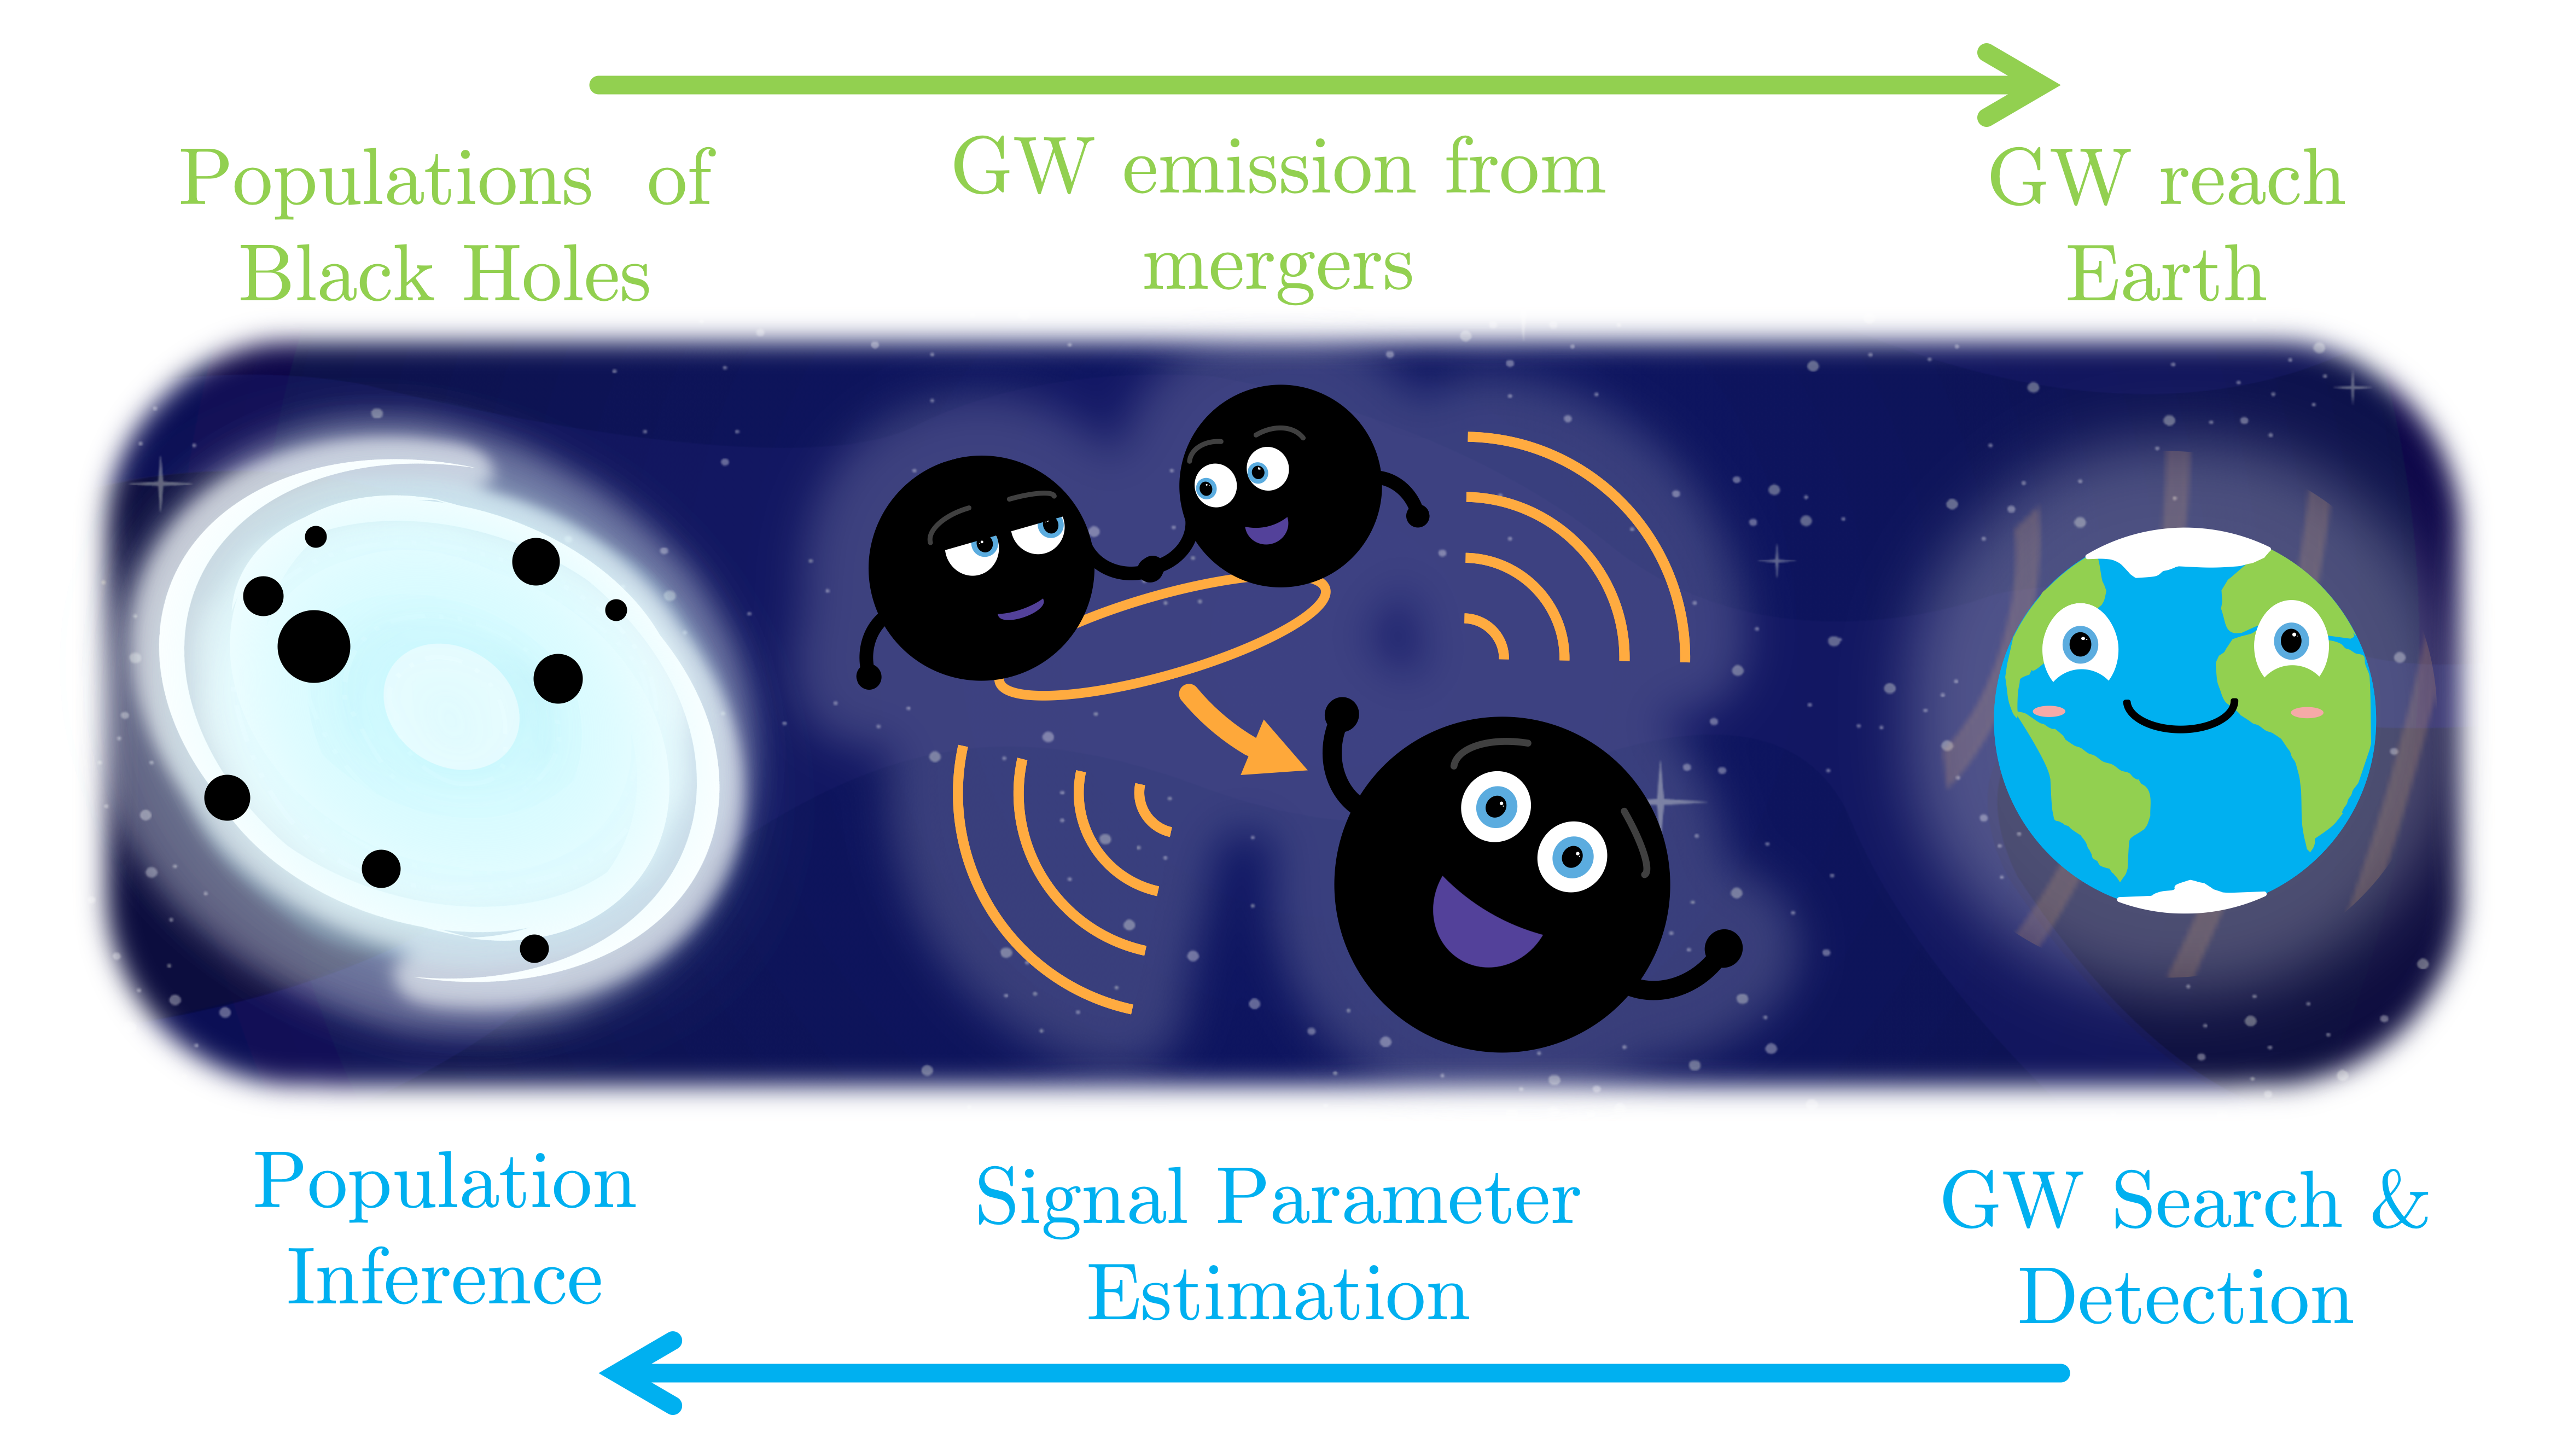
\includegraphics[width=1.1\linewidth]{src/figures/gw_pipeline.png}}
  \caption{\textbf{GW pipeline:} \todo{Remove faces from this schematic} }
  \label{fig:gw_pipeline}
\end{center}
\end{figure}

The following sections introduce the LVK collaborations efforts to (i) search for GW signals from compact binary mergers, (ii) decode the GW signal parameters that describe the merger, and (iii) study ``demographics'' of the merging black hole populations (each category and its goals are outlined in the schematic Figure~\ref{fig:gw_pipeline}).


\subsection{GW searches}  \label{sec:searches}

As LIGO records data, the data is immediately searched for generic, unmodelled GW transients and modeled GW signals using low-latency search pipelines. 
These searches can identify candidate GW events in near real-time timescales, enabling the possibility of performing follow-up electromagnetic spectrum observations~\cite{abbott2018prospects}.

The unmodeled gravitational wave searches, like the Coherent Wave-Burst (cWB) and BayesWave pipelines, are performed without prior information about expected signal waveforms and instead involve cross-correlating the LIGO and Virgo detector data. 
The cross-correlation is performed on the detector strain time series to look for excess power or bursts in the overlap region between the LIGO Hanford and LIGO Livingston detectors and between the LIGO Hanford and Virgo detectors, respectively \cite{LSC:2016}. 
Such methods are effective at identifying GW transients that can last for
$10^{-3}-10^{1}$s~\cite{abbott2016observing}. 
Unmodeled gravitational wave searches are powerful tools as they may help detect short-duration signals produced by unknown and known phenomena for which we have not yet developed good theoretical models~\cite{Abbott:2016blz}. 
For example, short-duration signals from high mass binary black hole mergers, supernovae, cosmic strings, and unknown astrophysical phenomena as described in~\citep{abbott2018prospects}.

While unmodeled searches look for the unknown,  modeled or targeted gravitational wave searches look for signals from known sources~\cite{abbott2016ligo}. 
Modeled searches for GW signals from the coalescence of compact binary coalescence (CBCs), such as `pyCBC'~\cite{biwer2019pycbc} and
`GstLAL' pipelines~\cite{sachdev2019gstlal},  use prior information about our expectations of GWs in searches. These searches compute the inner product between a gravitational waveform and the data stream and attempt to optimize the inner product by testing different waveforms. 
The different waveforms are chosen from a ``template-bank'' of potential waveforms, where each waveform corresponds to different signal parameters. 


\begin{figure}
\begin{center}
  \centerline{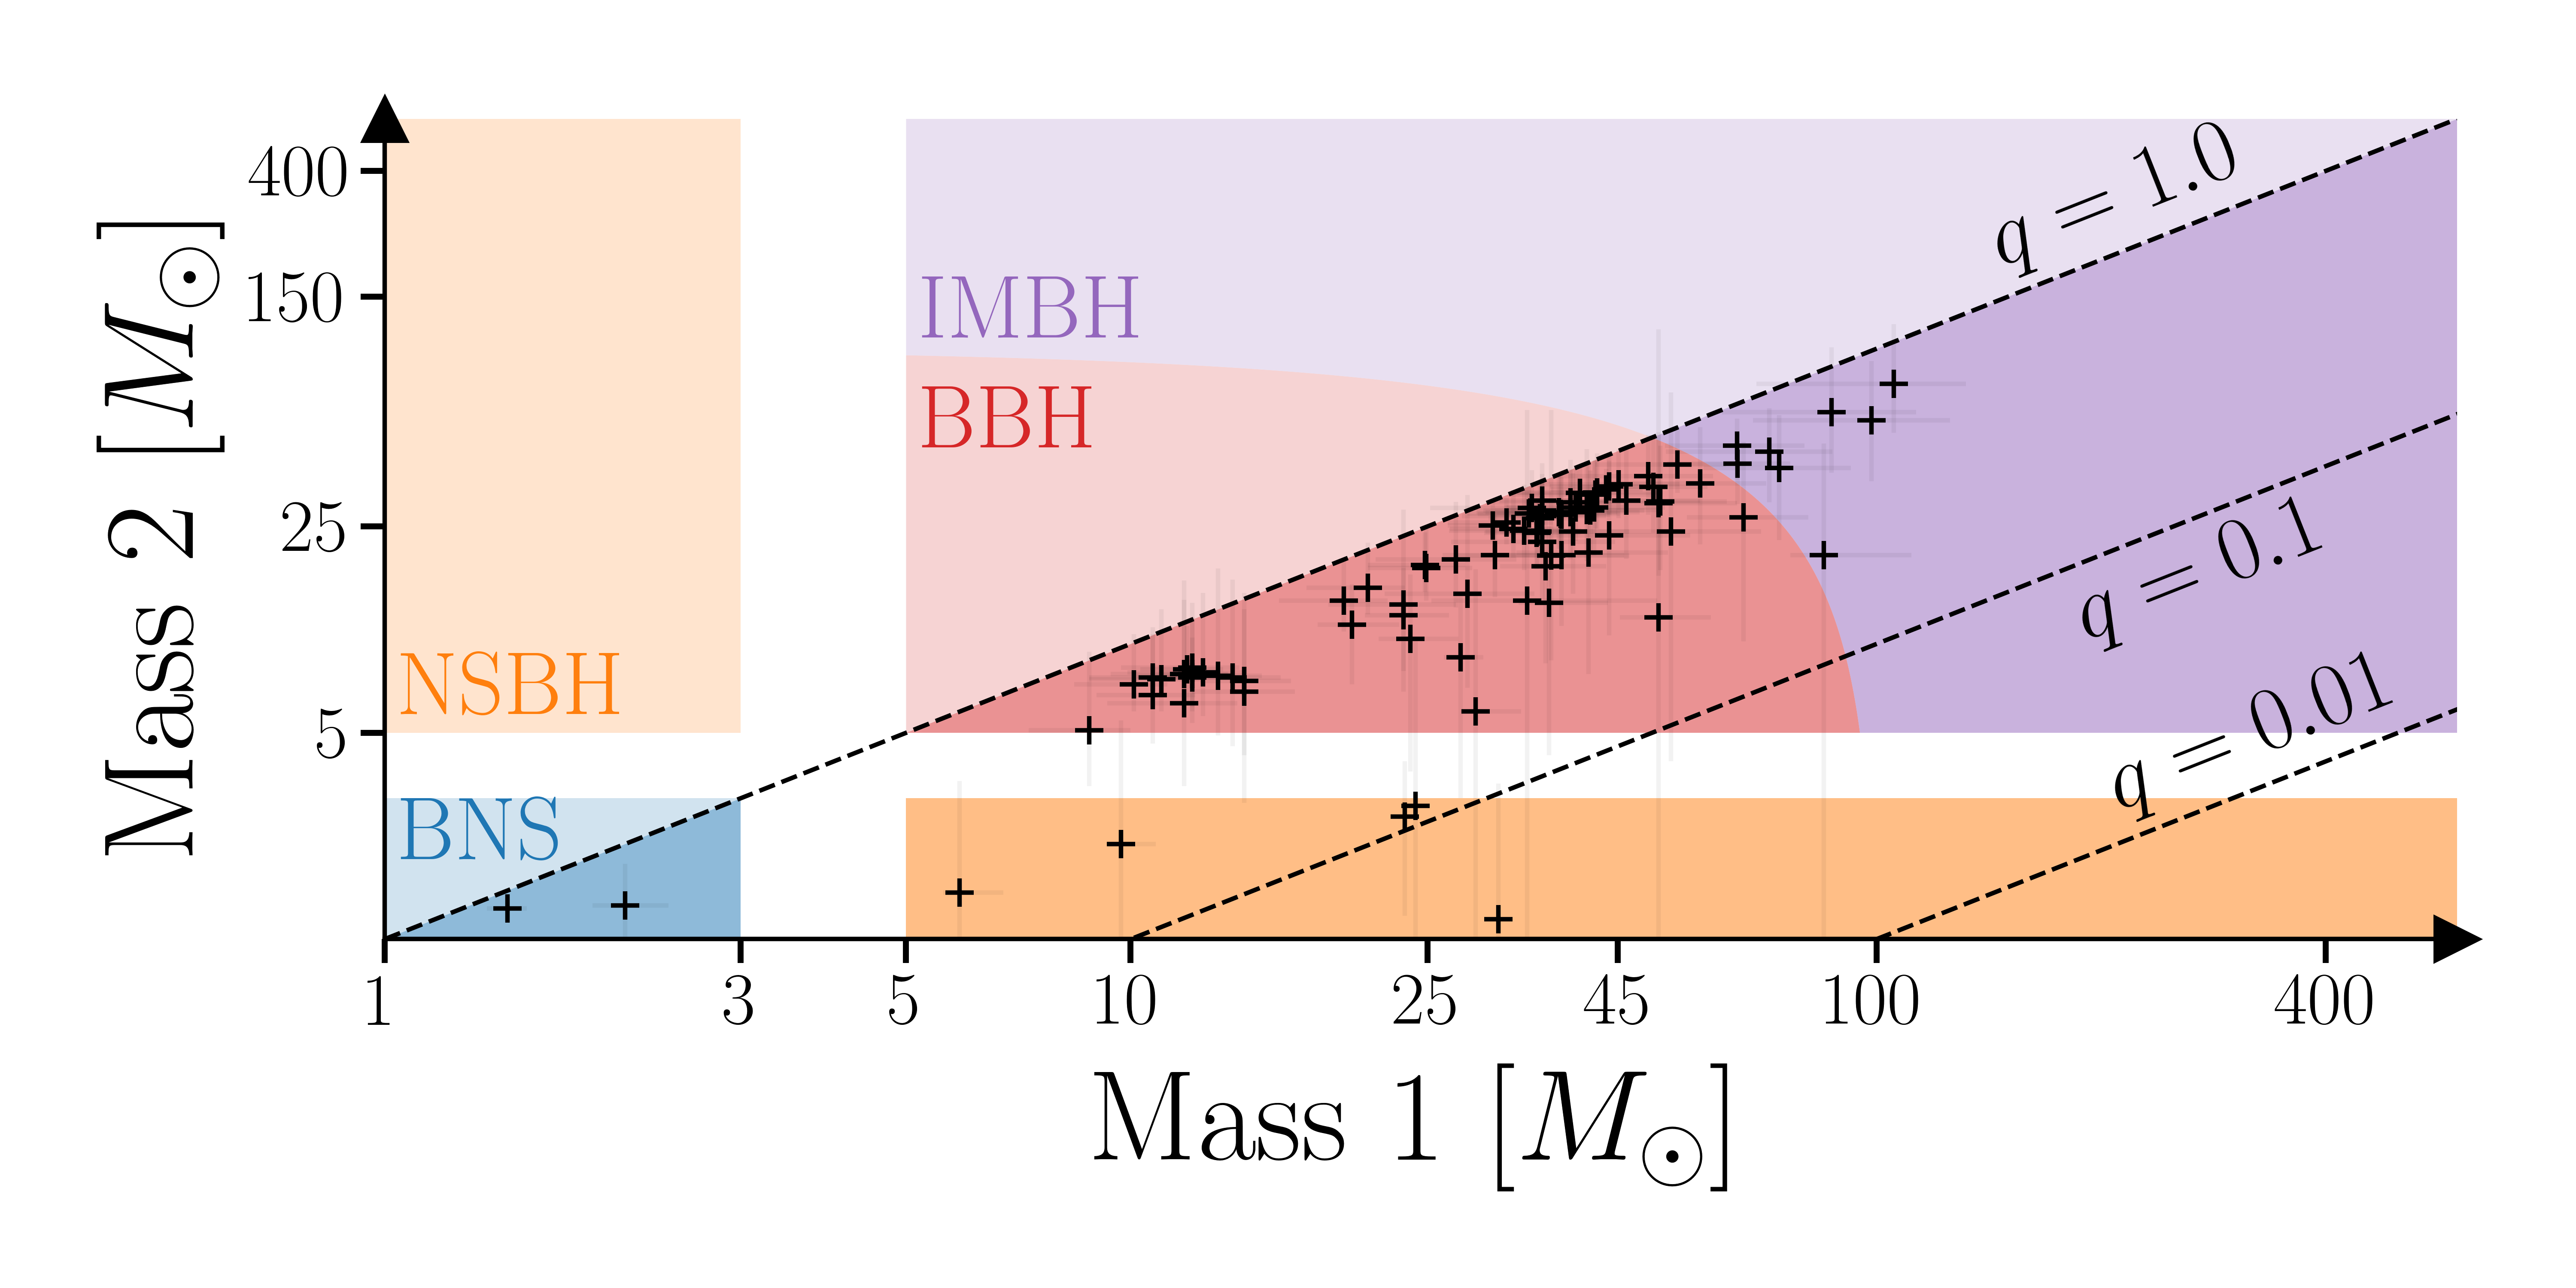
\includegraphics[width=1.1\linewidth]{src/figures/gw_catalog.png}}
  \caption{\textbf{CBC GW merger events:}  \github{https://github.com/avivajpeyi/cbc_gw_catalog_plotter}}
  \label{fig:cbc_mergers}
\end{center}
\end{figure}


These search methods have been able to successully identify more than 90 CBC GWs, whose masses are plotted in Figre~\ref{fig:cbc_mergers}.
If the detector data contained only gaussian noise and the occasional gravitational wave signal, these search pipelines would successfully identify all signals above some signal-to-noise ratio. 
Unfortunately, some instrumental noise artifacts (glitches) can also be found in the detector data. 
The search pipelines can mistake `glitches' as gravitational wave signals. 
Hence, the search pipelines also test signal coherence and compute `ranking statistics' to determine the statistical significance of candidates to prevent false positives. 

Efficient signal detection requires a ranking statistic that extracts the most information from the data to discriminate between noise and weak astrophysical signals.  
However, existing CBC searches are not optimal: they do not incorporate knowledge of all features that may distinguish GWs from noise. 
Moving toward an optimal statistic is a great challenge, but one toward a better ranking statistic may be to demand that foreground triggers in two or more detectors should be better described
as coherent gravitational-wave signals rather than incoherent glitches.
Importantly, it is not enough to provide some measure of coherence: one must also prove that an incoherent model is not more successful at
describing the data. 

The Bayesian coherence ratio, `BCR', proposed by \citet{bcr_paper} can help take a step towards this optimal statistic. 
As short-duration gravitational wave signals such as those from intermediate-mass black holes are the most challenging to distinguish from glitches, in Chaper~\ref{cp:imbh}, we investigate the usefulness of the `BCR' as a ranking statistic. 

\subsection{GW Signal Parameter Estimation}

The core of parameter estimation in gravitational waves is Bayes' theorem. 
Given a model with parameters $\theta$, some data $d$ and the \textit{likelihood} $\mathcal{L}(d|\theta)$ of the data given the model, Bayes' theorem states that the \textit{posterior probability} $p(\theta|d)$ of model parameters given the data is 
\begin{equation}
{p(\theta|d)} = \frac{\mathcal{L}(d|\theta)\pi(\theta)}{\mathcal{Z}}\ , \label{eq:bayeTheorem}
\end{equation}
where $\pi(\theta)$ is the \textit{prior} probability of the model parameters, and $\mathcal{Z}$ is the marginalized likelihood known as the
\textit{evidence}. 
The evidence is a single number that describes how well a model fits the data and is given by 
\begin{equation}
Z(d) = \int_\theta \mathcal{L}(d|\theta)\pi(\theta)d\theta\ .
\label{eq:evid}
\end{equation}
As the evidence is a probability of the data irrespective of model parameters, it is a valuable quantity to compare various models and determine which model better describes some data.

Using gravitational wave models and equation~\ref{eq:bayes}, astronomers can compute the posterior probability of gravitational wave model parameters given some data containing a gravitational wave signal~\cite{abbott2018prospects}.
However, as CBC GW models can use more than 11 parameters to describe a signal, evaluating the posterior probability for gravitational waves is computationally expensive. 
For example, consider evaluating the posterior probability at $10$ gridpoints for each of the $11$ GW parameters.
This case results in a huge number of $10^11$ points to evaluate the posterior.
Furthermore, one would need to use many more grid points to represent the continuous parameter space accurately.
Finally, gravitational wave models incorporate complex physics, so they can be computationally slow to evaluate. 
Altogether, evaluating the posterior overall points of parameter space is an insurmountable computational challenge.

An alternative way to estimate the posterior over a large parameter space is to utilize approaches such as Markov chain Monte Carlo (MCMC) and Nested Sampling to produce multivariate draws from the posterior. 
These methods can also be parallelized to speed up the inference process. 
For a detailed discussion on the parallelization of nested sampling and how it can boost gravitational wave inference, refer to Chapter~\ref{cp:pbilby}. 


\subsection{Interpretting GW signals}

After GW searches and parameter estimation pipelines  identify and characterise signals, astronomers can begin interpreting the inferred parameters .
Mass and spin inferences help determine where (eg isolated-space, globular clusters, or active galaxies) these binaries form and merge .
Each individual observation's inferred parameter can reveal the binary's formation pathway.

For example, consider the inferred parameters for GW190521 and GW190425. 
GW190521's parameters show that the signal originated from an asymmetric BBH merger with masses of $85^{+21}_{-14}M_{\odot}$ and $66^{+17}_{-18}M_{\odot}$ \citep{Abbott:2020tfl}.
The remnant object was the first direct detection of an IMBH with a mass surpassing the pulsational-pair instability mass gap.
Due to its large initial masses, some believe that this may be a second-generation merger and hence is improbable to be a field-merger. 
On the other hand,  parameter estimation of GW190425 suggests the event's binary had a non-circular orbit, indicating it may have come from a globular cluster.

In a similar vein, the community has recently been discussing GW151226. 
Initial research concluded that GW151226 was the result of the merging of two BHs with conventional masses and spins, as seen in Figure~\ref{fig:gw151226_cases} (case A).
However, recent work suggest that the GW emerged from a peculiar system: asymmetric BBH merger with even spins misaligned (case B).

%% GW151226 Figure
\begin{figure}
\begin{center}
  \centerline{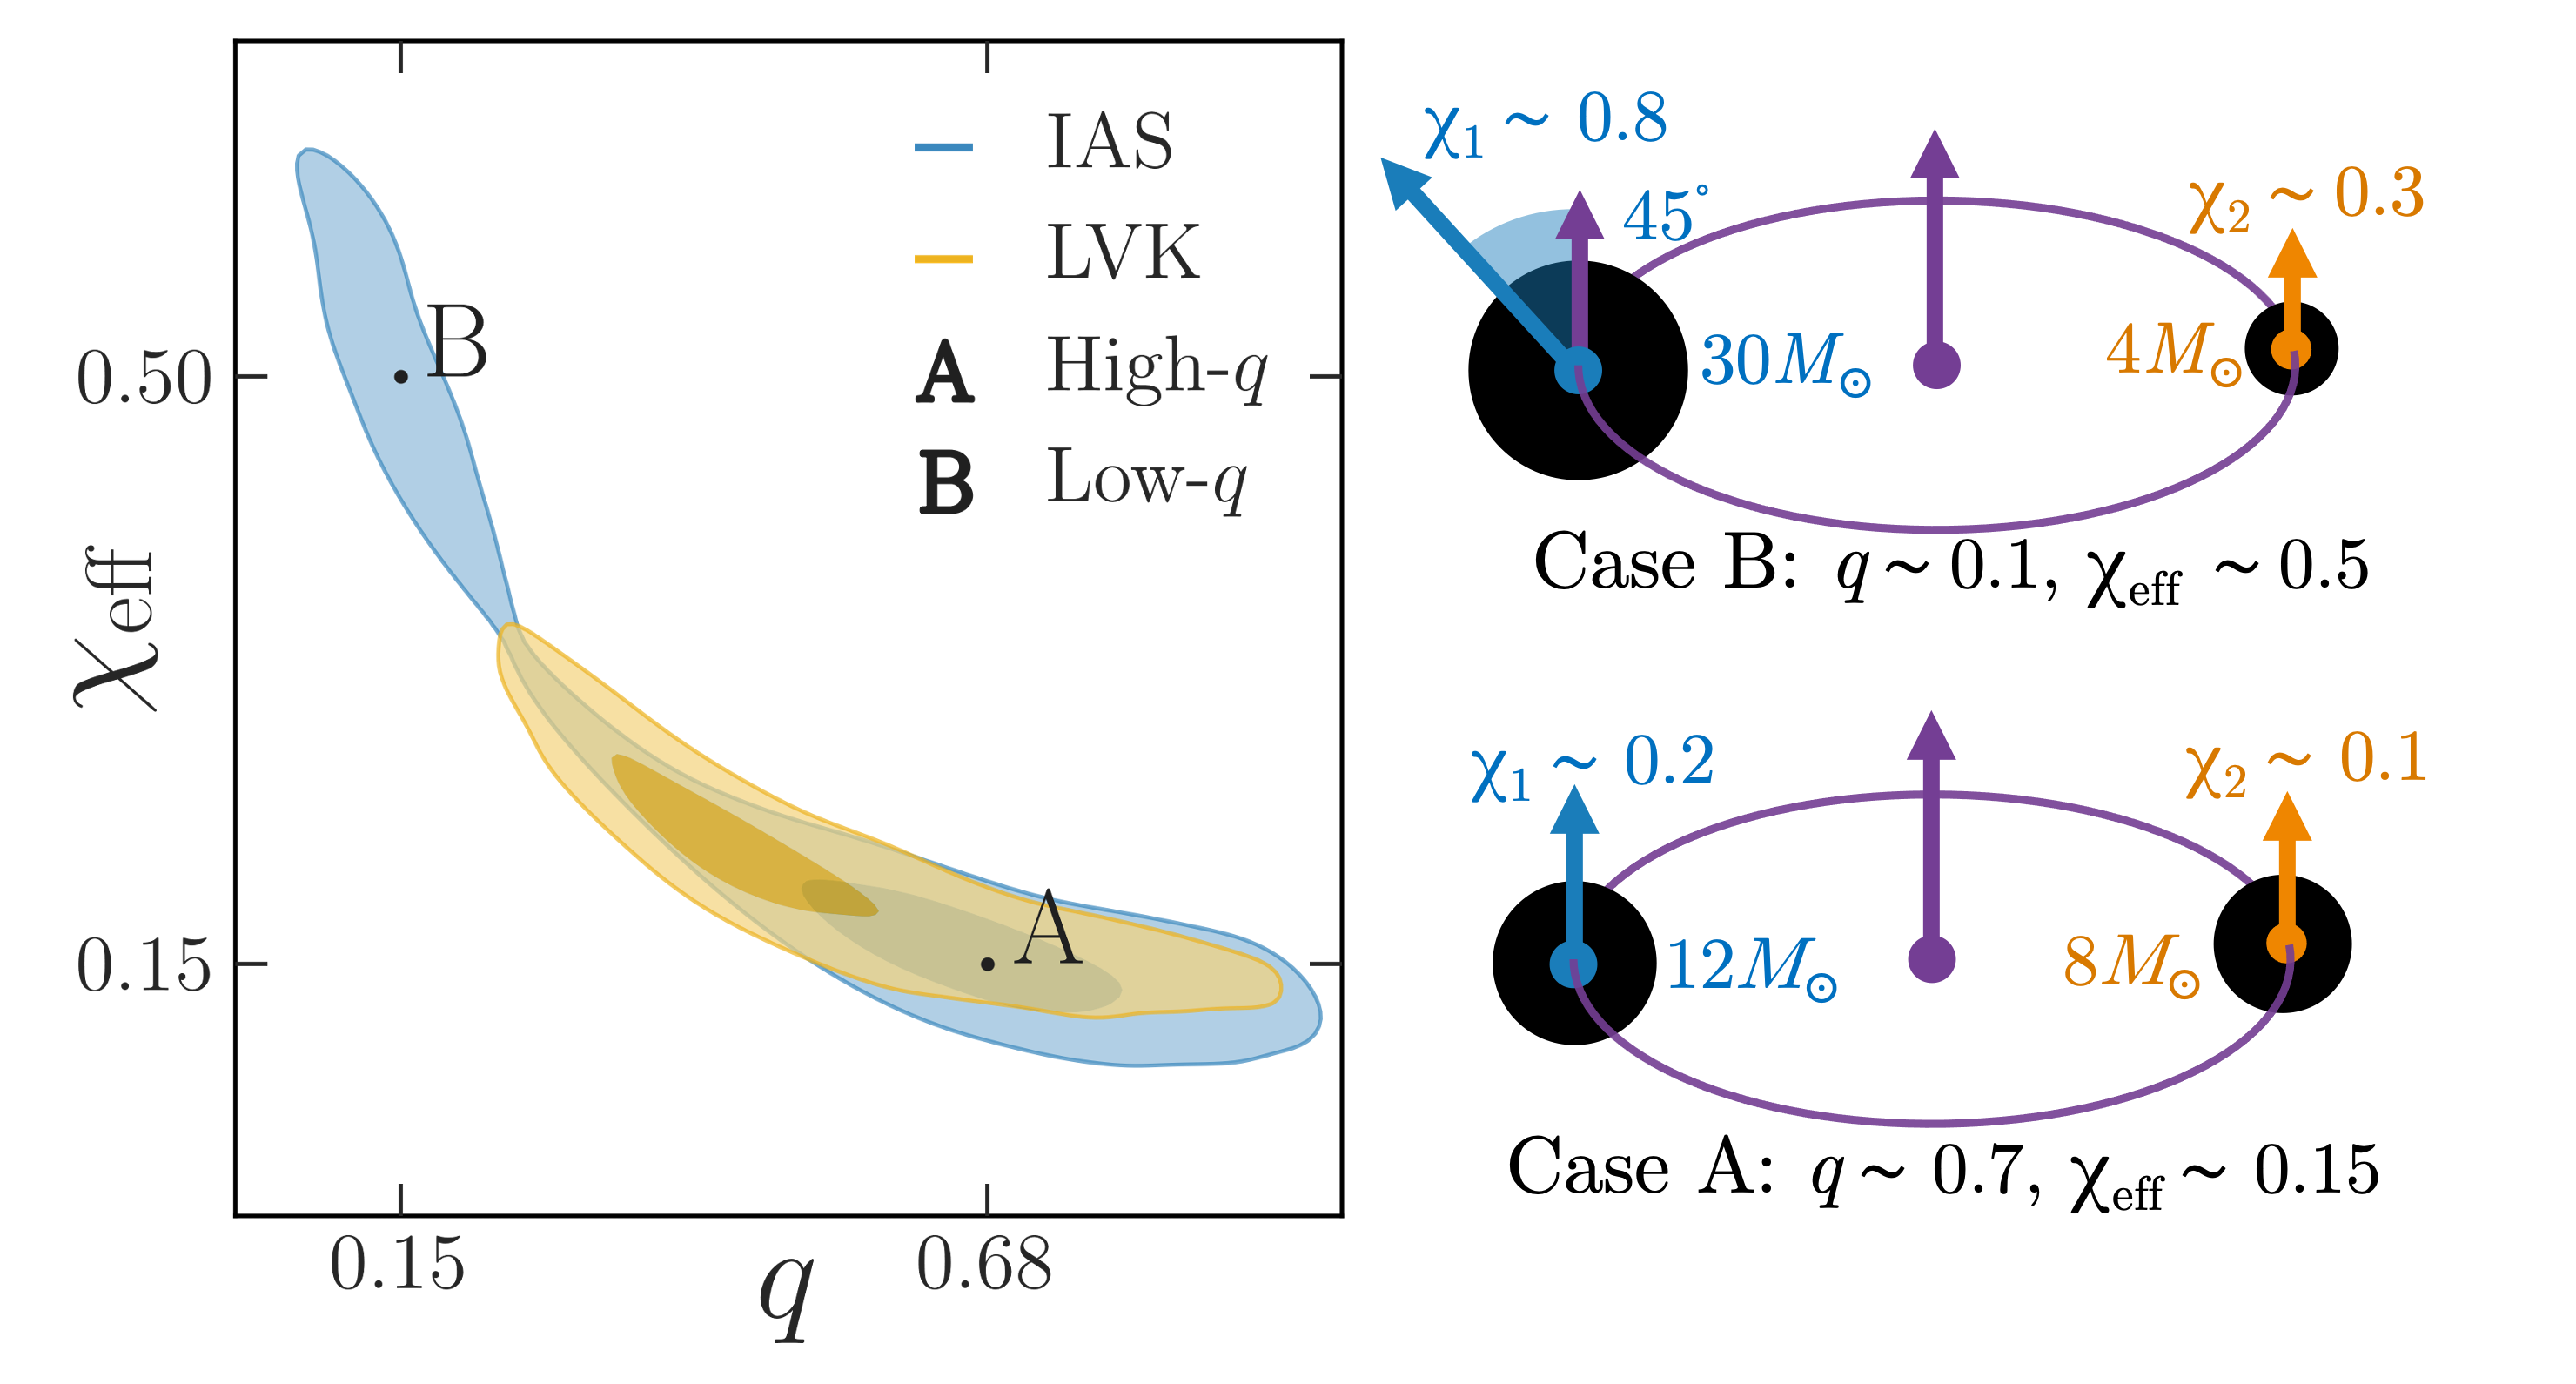
\includegraphics[width=1.1\linewidth]{src/figures/gw151226_cases.png}}
  \caption{\textbf{GW151226 Cases:}  }
  \label{fig:gw151226_cases}
\end{center}
\end{figure}

It's uncertain which of these cases is most likely, making it difficult to establish this event's formation channel.
Chapter~\ref{cp:deep_followup} presents a ``deep follow-up'' tool to determine which case is  more probable.
It employs Bayesian model selection to evaluate the posterior odds of two points by computing the points marginal likelihood.
The posterior odds for case A versus B are near 1, reflecting that it is valid to interpret GW151226's binary to have been from either case.

\subsection{GW population inference}

With many GW events, astronomers can also study the ensemble properties of merging systems, such as how masses and spins of all detected BHs are distributed, using hierarchical inference techniques.
The LVK has used several hypotheses in hierarchical inference studies to map ensemble mass and spin distribution features to astrophysical processes  described by stellar evolution and population synthesis models.
Recent work on the black hole spin population, for example, has looked into computing the fraction of signals expected to result from isolated-field binary mergers versus dynamical binary mergers.
In Chapter~\ref{ch.agn}, we look into yet another binary merger channel: the active galactic nuclei (AGN) channel.
AGNs are promising environments for the assembly of merging binary black hole systems with large masses (e.g. GW190521~\cite{gw190521_agn}), asymmetric masses (e.g. GW190521~\cite{gw190425_agn}), and a variety of spin configurations~\cite{agn_spin_population_models}. 

\begin{figure}
\begin{center}
  \centerline{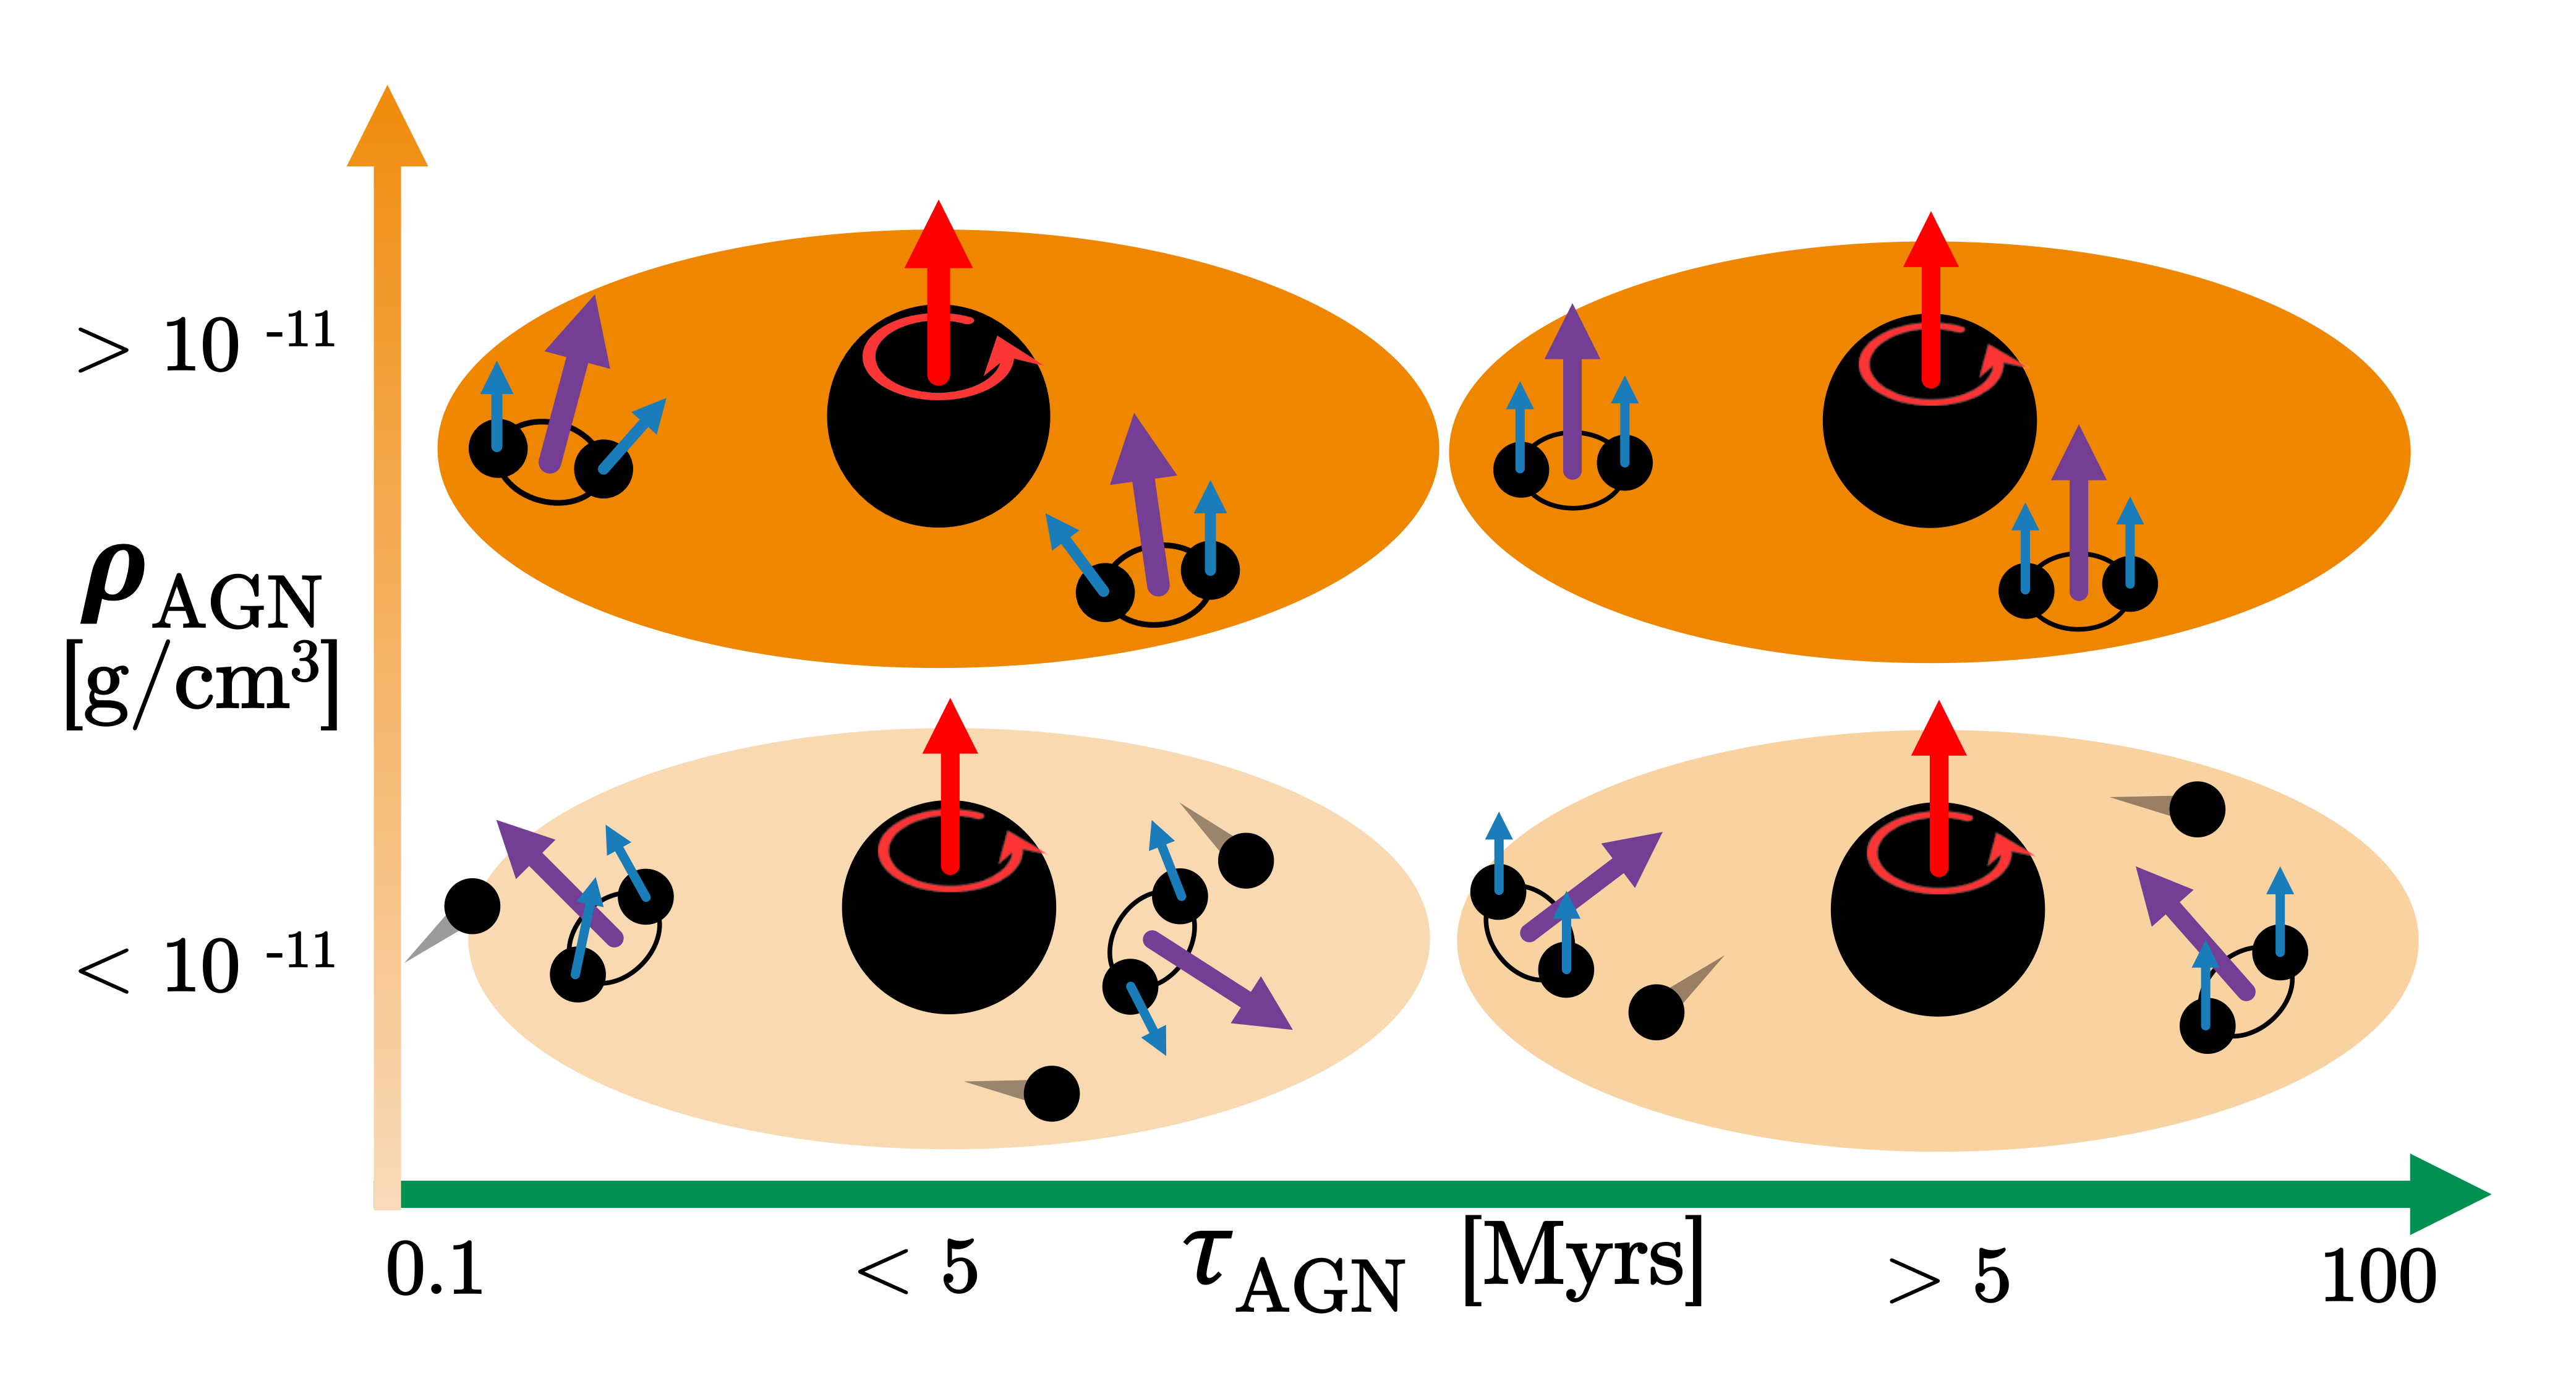
\includegraphics[width=1.\linewidth]{src/figures/agn_spins.png}}
  \caption{\textbf{AGN BBH-spins:} Different AGN age $\tau_{\rm AGN}$ and density $\rho_{\rm AGN}$ values can lead to different binary black hole spins. }
  \label{fig:agn_spins}
\end{center}
\end{figure}


In Chapter~\ref{ch.agn} we draw on simulations of BBH systems in AGN to propose a phenomenological model for the distribution of black hole spins of merging binaries in AGN disks. 
The model incorporates distinct features that make the AGN channel potentially distinguishable from other channels such as assembly in the field and in globular clusters. 
The model parameters can be mapped heuristically to the age $\tau_{\rm AGN}$ and density $\rho_{\rm AGN}$ of AGN disks. 
A schematic illustration of the model is presented in Figure~\ref{fig:agn_spins}. 
In the Figure's top right corner where the AGN is old and dense, the BBH orbital angular momentum and component BH spins align with the central SMBH spin. 
Coversly, in the lower left where the AGN is young and dilute, all spins are missaligned. The other two corners represent unique spin orientations described in further detail in Chapter~\ref{ch.agn}.
We estimate the extent to which these different populations of binaries in AGNs can be distinguished.
If the majority of merging black holes are assembled in AGNs, future gravitational-wave observations may provide insights into the dynamics of AGN disks.

\section{The hunt for exoplanets}

Humans have long sought for exoplanets, planets beyond our solar system, to answer questions like how did the Earth form, are we alone in the universe, and are there other planets like ours out there? 
Similar to the 


In recent years, advances in technology have allowed us to find and study many exoplanets. We have now found thousands of exoplanets, and we are learning more about them every day.

There are many different types of exoplanets, and they can be very different from the planets in our solar system. Some exoplanets are very large, while others are very small. Some exoplanets are very close to their star, while others are very far away. And some exoplanets are very hot, while others are very cold.

Despite these differences, there are some things that all exoplanets have in common. All exoplanets orbit a star, and all exoplanets are made of the same basic materials as the planets in our solar system.


This section reviews the hust for exoplanets and some of what we have learned from the exoplanets we have founds so far. 

\begin{itemize}
    \item History: We have looked for exoplanets for along time, first few exoplanets found 
    \item Plot of detectiions vs time
    \item categories of exoplanets + Habitable zone
    \item radius + mass info relations of exoplanets 
    \item Kepler project -- cone in sky
    \item now, TESS project, helped us find many more, survey satellite for nearby stuff
    \item gist of search pipeline + parameters provided
    \item our work 
\end{itemize}

\section{Explanets from the 90s to now}


% Jay paper https://arxiv.org/pdf/1604.03092.pdf

Sometimes scientists stumble upon discoveries. 
The first discovery of an exoplanet was one such stumble.
While the globe was reeling from the outbreak of WW1, Walter Adams recorded the spectrum of a white dwarf star on a glass plate. 
This star's spectrum contains unusual heavy elements including magnesium and iron. 
As these would not naturally form on the planet, these pollutants must have come from the shattered remains of an exoplanet. 
Hence,making this the first evidience for an exoplanet. 
Unfortunately, Adams didn't realise this, and his discovery remained kept in the archives until 2016 — when Jay Farihi unearthed it.

So, the credit for the first exoplanet goes to astronomers Aleksander Wolszczan and Dale Frail.
In 1992, these scientists nooticed that the pulsar PSR B1257+12 had periodic variatinos in its pulses.
After intensive study, Wolszczan and Frail came up with an explanation for why that was: it had two planets around it. One was three and the other four times the mass of Earth, and they rotated around every 67 and 98 days, rounded up.
However this was a very perplexing planetary system to the astronomers, 

normally When a star explodes, usually the planets in that system are destroyed or flung out by a shockwave. But after the violence settles down, the gas and dust can recondense. This, in effect, means that the three planets in B1257 may be made out of parts of the planets that came before them. Given the extreme radiation in these systems, almost no one has ever thought that the B1257 system could host life.

So, while the 1992 discovery was major news, it meant astronomers had the first verified planets around another star, but no proof of planets around a main sequence star like the Sun. That kind of confirmation was still a few years away.



Reportedly, his find was a chance coincidence. Out of a catalog of radial velocity signatures, he chose an F-type star called 51 Pegasi, roughly 50 light-years distant. He was trying to calibrate his planet finding code, opting for the star as one of a few promising candidates. It fell into place that night, a strong signal roughly every four days.

Measurements placed its minimum mass near Jupiter —  meaning the object was without a doubt a planet. While astronomers considered it possible to have such periods, it wasn’t necessarily expected to find one in such a short period. “At this time, I was the only one in the world who knew I had found a planet,” Queloz told the BBC in 2016. “I was really scared, I can tell you.”


This discovery was followed in 1995 by the discovery of 51 Pegasi b, the first exoplanet found to be orbiting a normal Sun-like star. The work of Swiss astronomers Michel Mayor and Didier Queloz used the radial velocity technique to prove the existence of the planet orbiting its parent star every 4.23 days. They used the ELODIE spectrograph (see Figure 2) at the Observatoire de Haute Provence in France. 51 Peg b has a similar mass to Jupiter but is much closer to its star, being more than 7 times nearer than Mercury is to our Sun. This affords it the understated designation of a 'hot Jupiter'.


he early days of exoplanet detections were marked by their focus on star-by-star analyses, almost always through radial velocity, making radial velocity one of the most successful methods for finding exoplanets, discovering 746 worlds as of March 2018. Compare that to 90 found through some form of direct imaging (which is limited to large, hot, and young planets) or 67 through microlensing — chance happenstance when a heavy object passes in front of a background star and acts like a giant magnifying glass. Those are the third and fourth most successful methods for finding exoplanets.

But far and away the most successful approach has been the transit method of finding exoplanets. It’s found 2,789 in all within the same timeframe as the radial velocity headcount. There are 3,705 planets out there, so transiting planets make up 75 percent of all planets discovered. But around 2,648 of those 2,789 planets have been found by one spacecraft: Kepler.

If you take out the worlds discovered by NASA’s Kepler mission, we have only 1,000 planets to work with. That’s because Kepler served as a survey of just one small patch of sky, counting as many planet transits as it could. Previous surveys dealt with a few dozen stars at a time — if that. Kepler, if nothing else, showed that planets weren’t rare at all, and there are millions — or trillions — out there, waiting for our discovery.

Astronomy continued to do its thing for a few more years, with exoplanets popping up here and there after a series, of dedicated studies. And then in 2009, the game changed completed with NASA’s launch of the Kepler Space Telescope.

Kepler was an exoplanet hunter extraordinaire, dedicated to finding planets orbiting other stars. And it did a fantastic job at it, generating a catalog of thousands of worlds over the course of its nearly 10-year lifespan.

With Kepler, astronomers found planets bigger than Jupiter, and ones smaller than Mercury. They even found planets bigger than Jupiter orbiting closer to their parent star than Mercury does in our solar system. They found crazy worlds that rain iron, and others locked in ice. Other missions found exoplanets around our nearest neighbor star, Proxima Centauri, and a cache of seven Earth-like planets in the TRAPPIST-1 system 40 light-years away.

New surveys are on the case, like TESS, NASA’s Transiting Exoplanet Survey Satellite, and ground-based observatories around the globe. Exoplanets are providing a wealth of information about how planets and solar systems form throughout the galaxy…and the possibility of another habitable world is just too tantalizing to pass up.

But it was only in 1995 that astronomers spotted the first planets orbiting sunlike stars outside of our solar system.

In the last decade, in particular, the number of planets known to orbit distant stars grew from under 100 to well over 2,000, with another 2,000 likely planets awaiting confirmation. Most of these new discoveries are due to a single endeavor 


The first extrasolar planet discovered was found in 1995 orbiting the star 51 Pegasi.1 At that time, most astronomers presumed we would eventually discover many planets manifesting characteristics virtually identical those in our solar system.

To date, astronomers have discovered 854 planets outside the solar system for which they have also measured orbital and physical parameters. Not even one of these planets matches the characteristics of any of the solar system’s planets. The only one that comes close is Upsilon Andromedae e. Its mass compared to Jupiter’s is 1.06+ (because the inclination of Andromedae e’s orbit is not known, only a minimum mass has been determined). Its distance from its host star compared to Jupiter’s distance from the Sun is 1.01.



% https://sites.pitt.edu/~stepup/ExoplanetHistory.html


\begin{figure}
\begin{center}
  \centerline{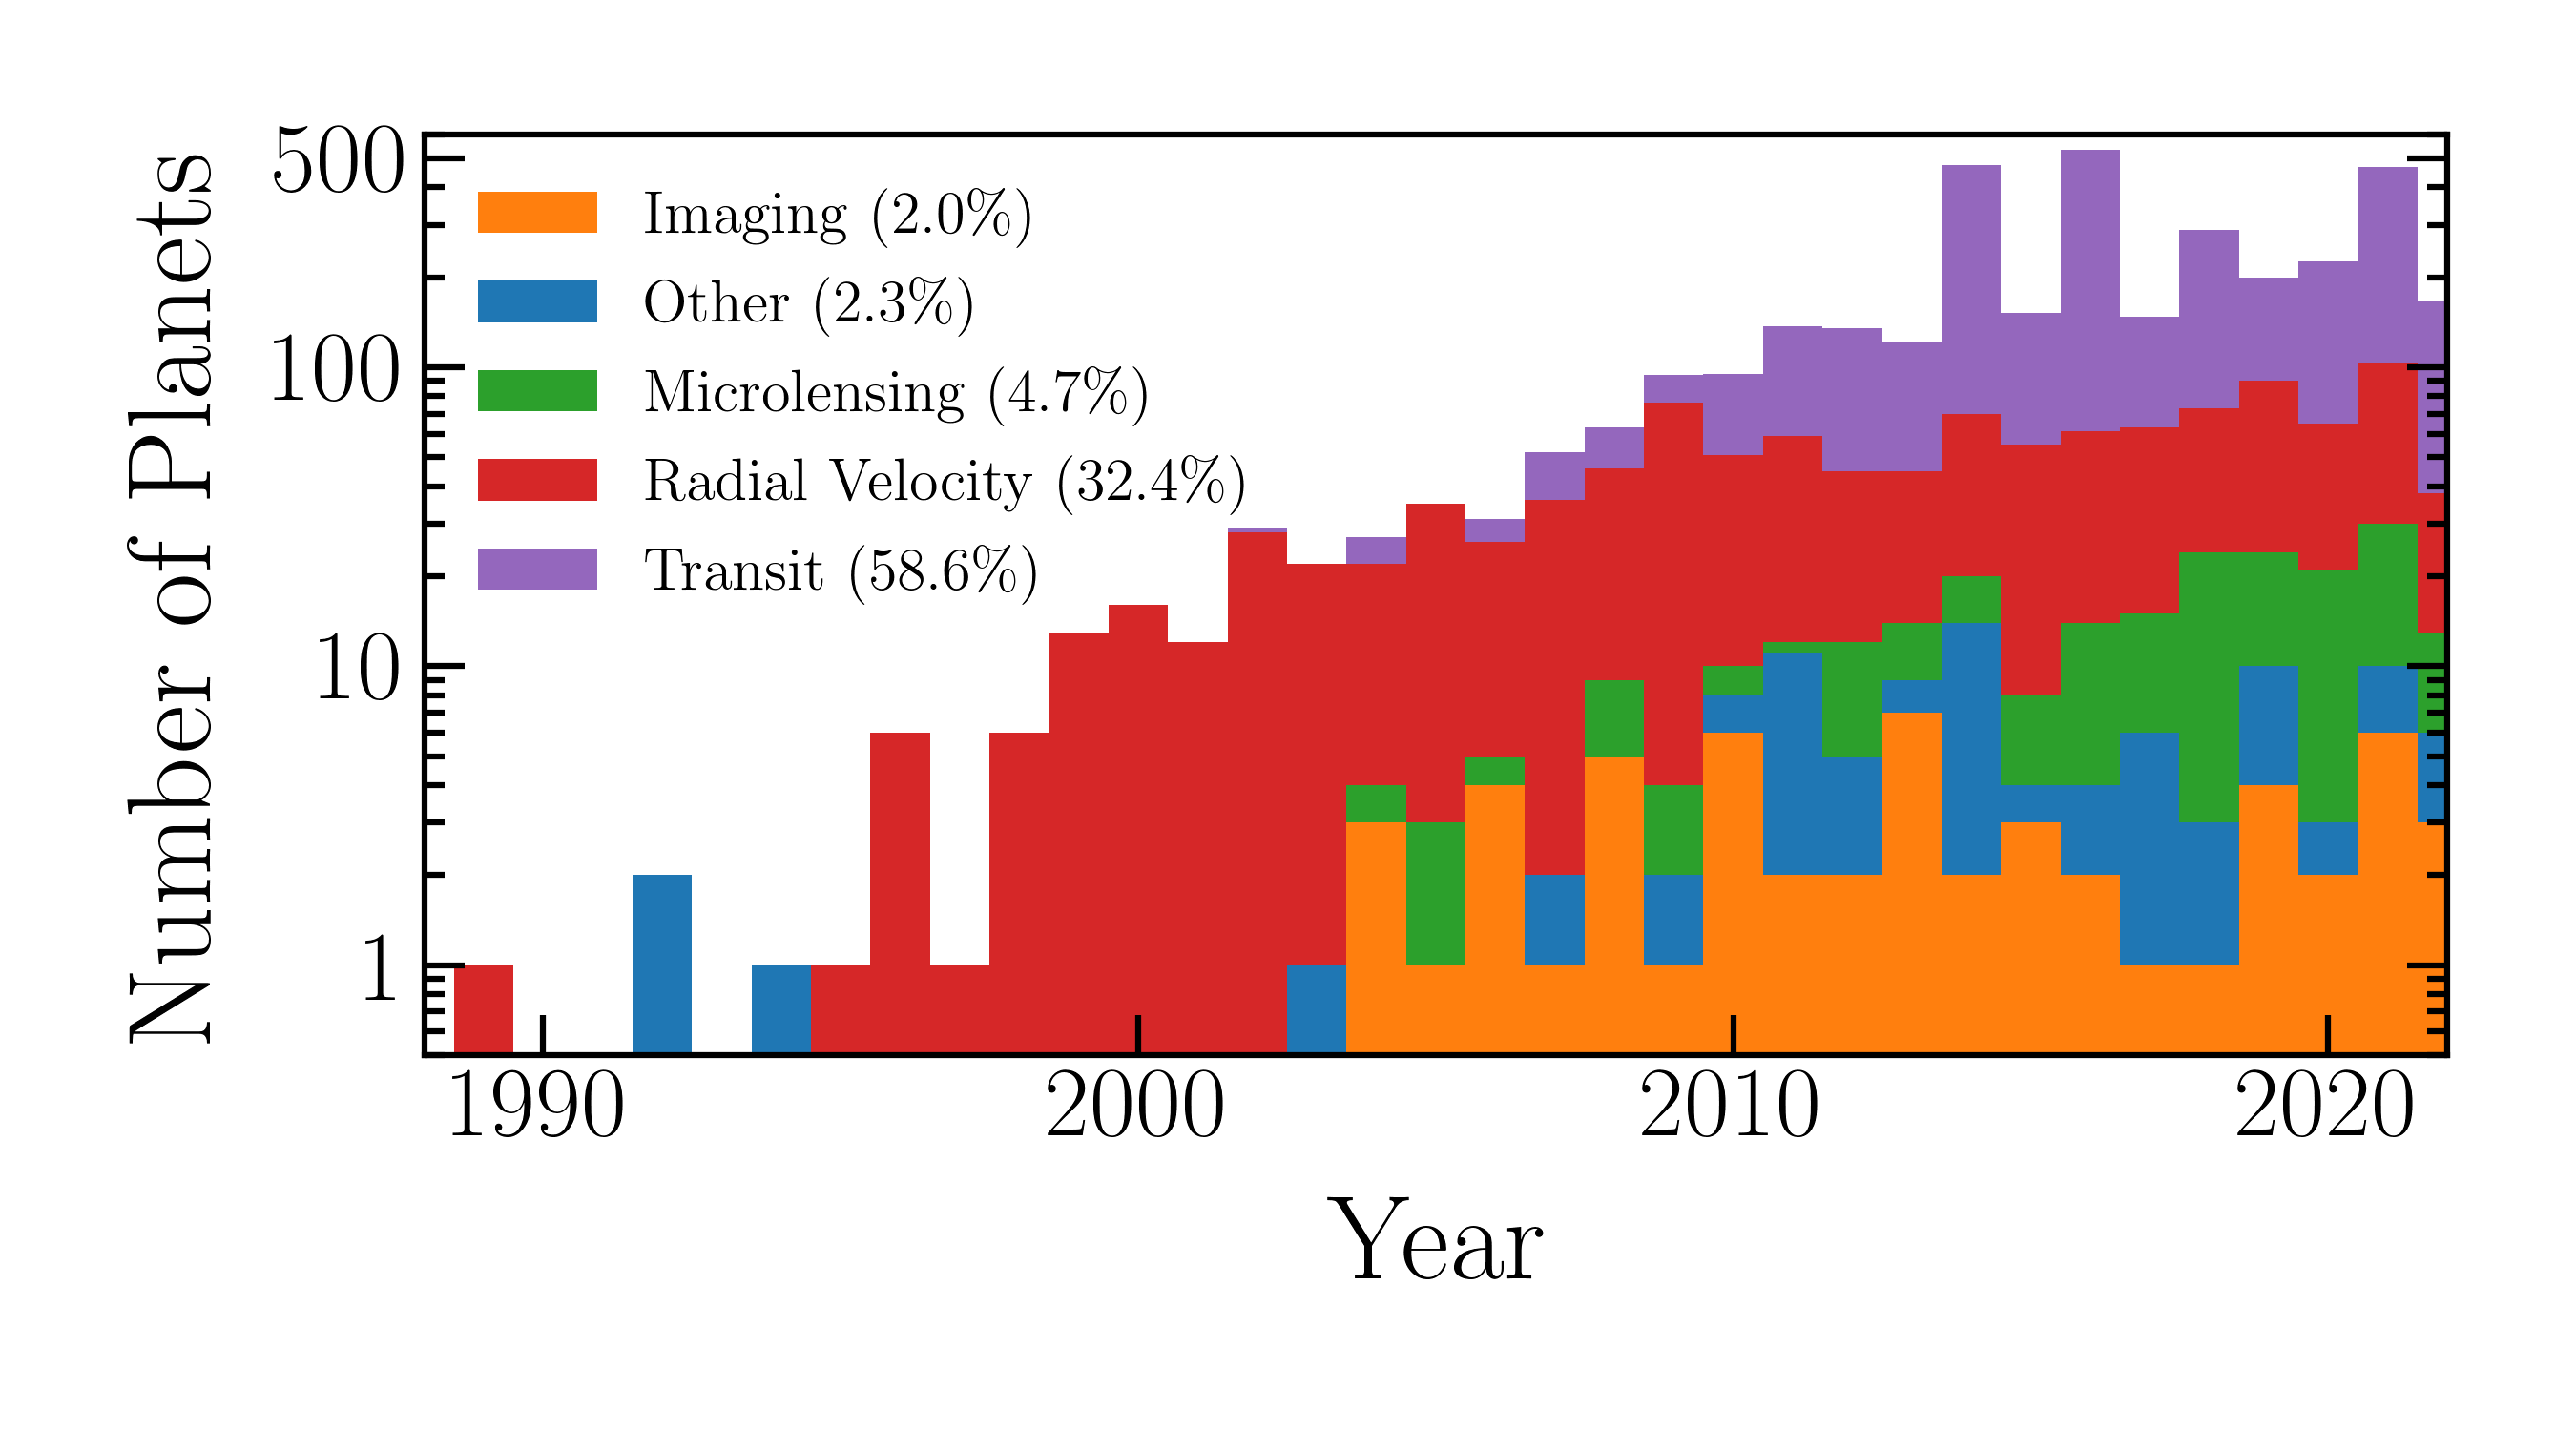
\includegraphics[width=1.\linewidth]{src/figures/confirmed_planets_vs_time.png}}
  \caption{\textbf{Exoplanet detections over time:}  \github{https://github.com/avivajpeyi/exoplanet_catalog_plotter}}
  \label{fig:exo_detections_over_time}
\end{center}
\end{figure}


\begin{figure}
\begin{center}
  \centerline{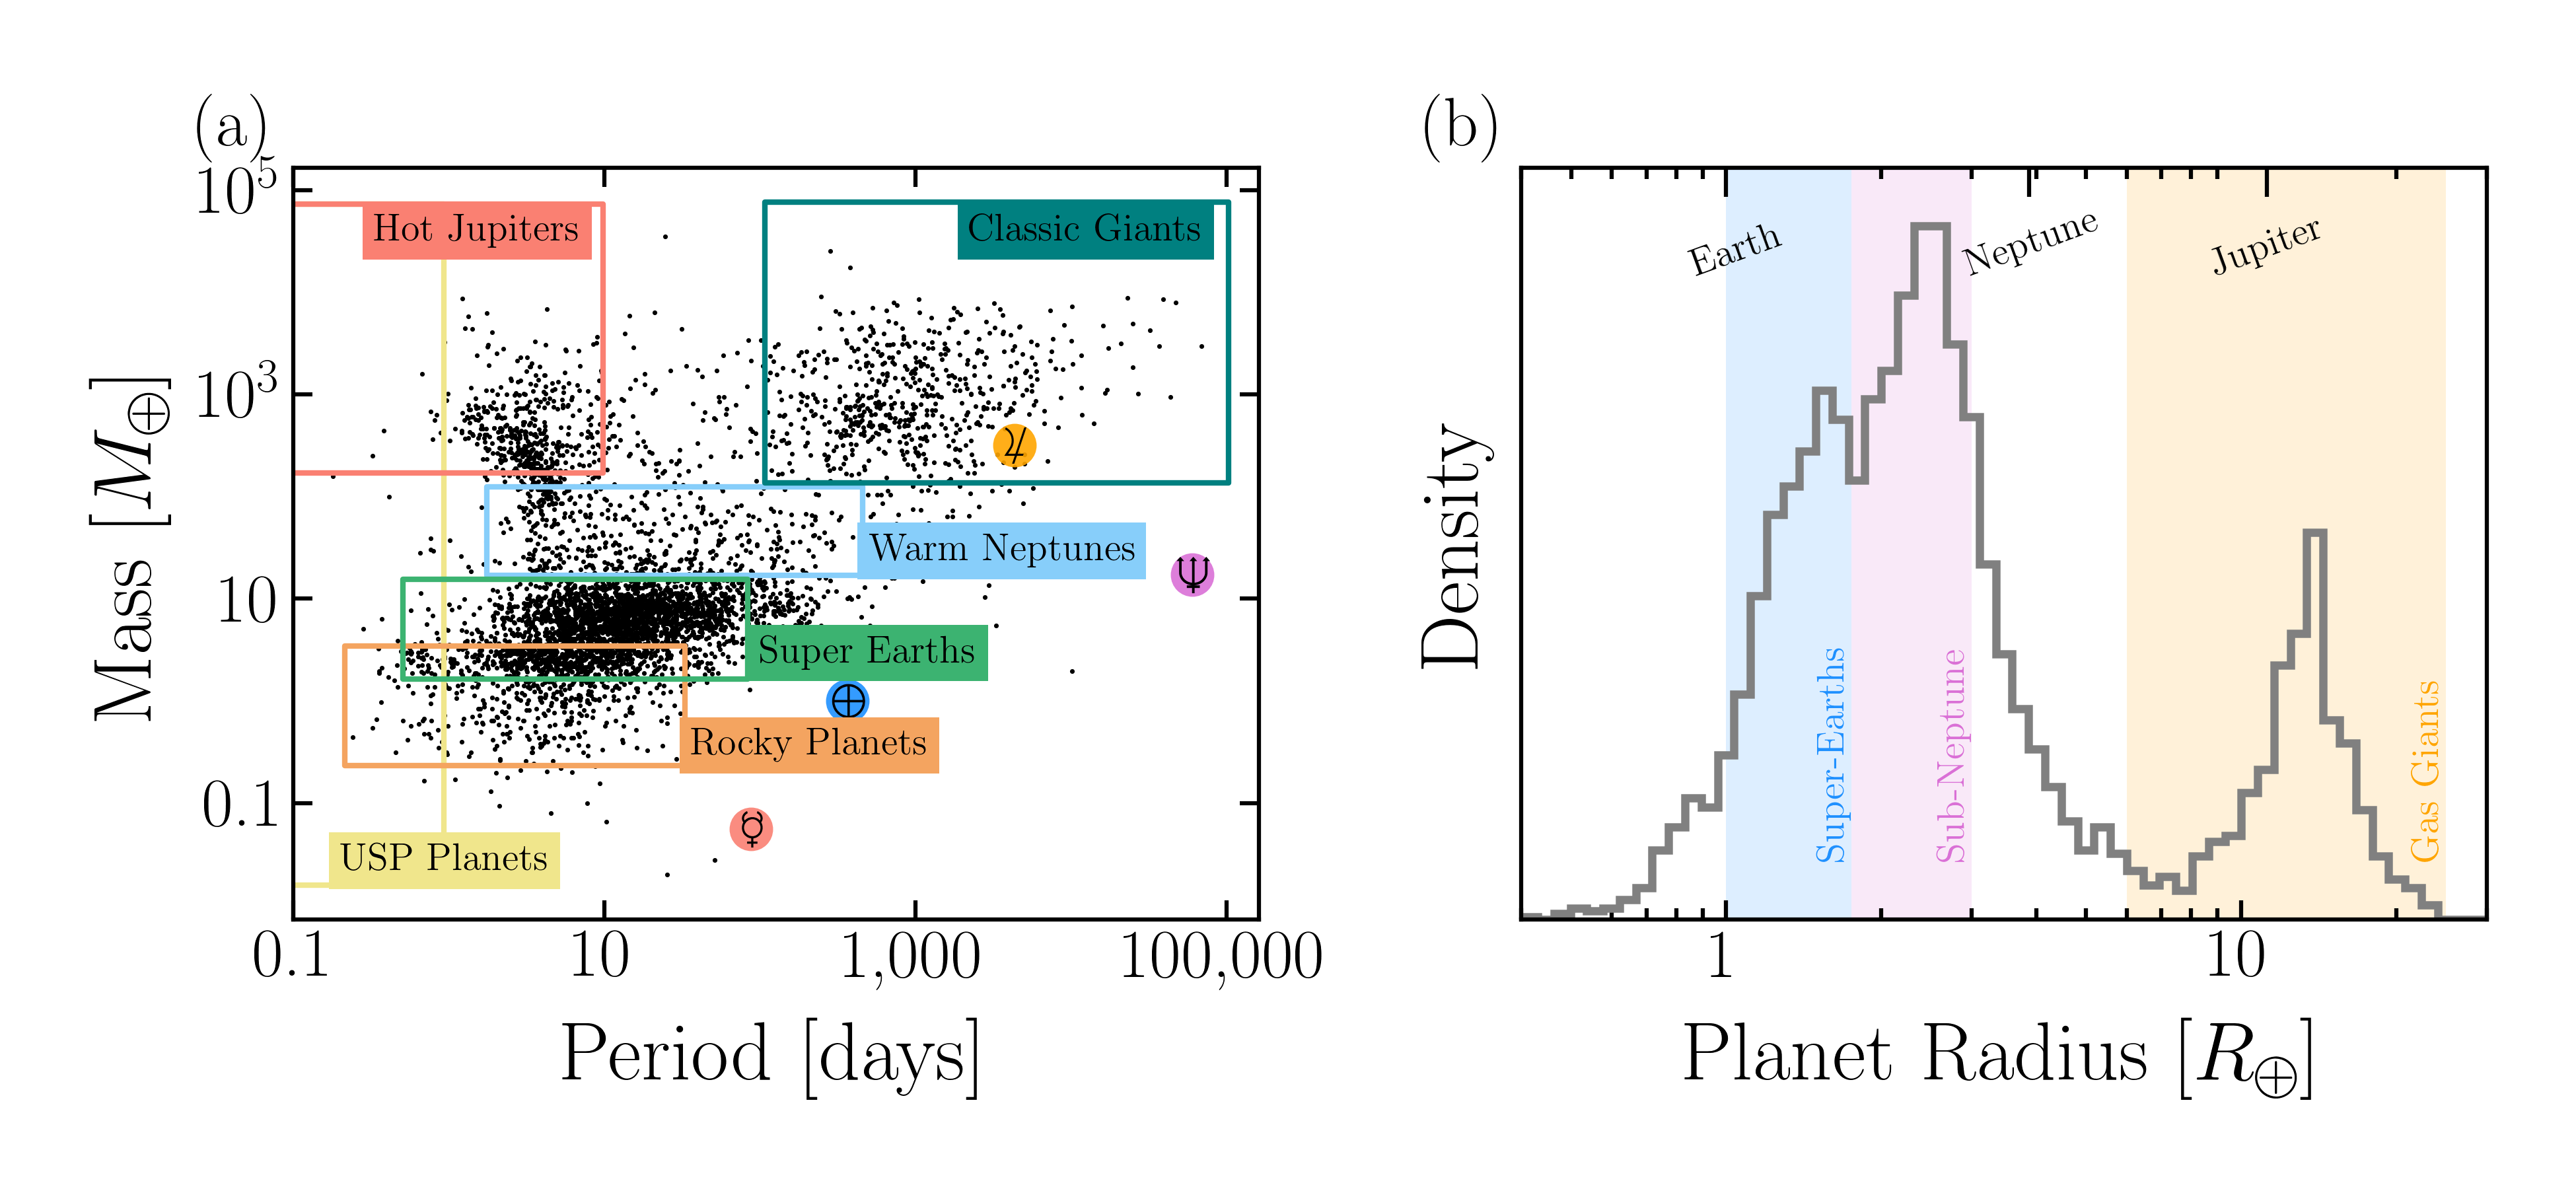
\includegraphics[width=1.\linewidth]{src/figures/scatter_categories.png}}
  \caption{\textbf{Exoplanet Categories:}  \github{https://github.com/avivajpeyi/exoplanet_catalog_plotter}}
  \label{fig:exo_categories}
\end{center}
\end{figure}

exoplanets with measured diameters and masses. Rocky planets form a tight line (lower left), but super-Earths/mini-Neptunes have widely varying atmospheres and densities. At Jupiter’s size, increasing mass no longer increases the diameter of a planet (upper right). Most of Kepler’s discoveries would be in the super-Earth/mini-Neptune region, but few of them have measured masses, so they do not appear here. This graph was originally published in "T


\begin{figure}
\begin{center}
  \centerline{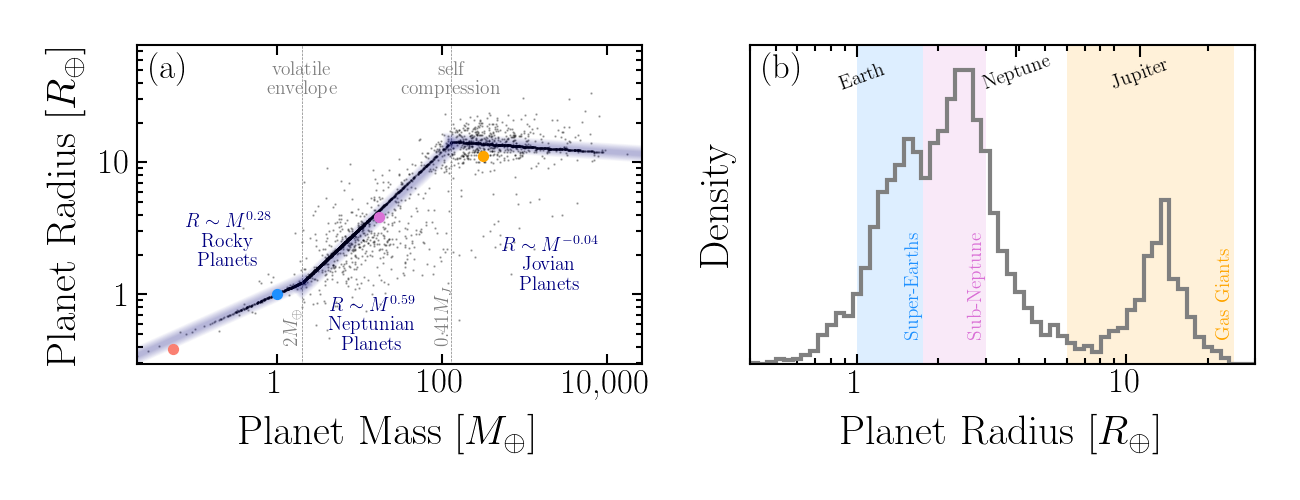
\includegraphics[width=1.\linewidth]{src/figures/radii_and_mass_relations.png}}
  \caption{\textbf{Digging into exoplanet mass and radius distributions:}  \github{https://github.com/avivajpeyi/exoplanet_catalog_plotter}}
  \label{fig:exo_mass_radius_relations}
\end{center}
\end{figure}




% Rocky vs gas 
% http://backalleyastronomy.blogspot.com/2013/07/au-dela-de-neuf-cents-exoplanetes.html
